% !TEX root = ../gnss_interference_resistant_thesis.tex
\documentclass[main.tex]{subfiles}

\begin{document}

\subsection{KerberosSDR imtuvas}\label{sec:kerberossdr}

KerberosSDR yra SDR imtuvas gebantis priimti signalus dažnių ruože nuo $24\ \mathrm{MHz}$
iki $1,7\ \mathrm{GHz}$, ADC yra 8 bitų ir veikia iki $2,4 \mathrm{MHz}$ diskretizacijos dažnio
\cite{kerberossdr}.
KerberosSDR yra sudarytas iš 4 RTL-SDR imtuvų. RTL-SDR yra atviro kodo imtuvai, padaryti iš
DVB-T standartinių imtuvų, kurie yra lengvai prieinami. KerberosSDR imtuvas
gali būti naudojamas krypties nustatymui, pasyviniam radarui ar spindulio formavimui.

KerberosSDR imtuvas turi integruotą plačiajuostį triukšmų generatorių, kuris leidžia
sinchronizuoti imtuvų darbą, atlikus kalibravimą radijai gali veikti kaip koherentinis imtuvas.
Vienas iš KerberosSDR trūkumų, yra reikalavimas atjungti antenas prieš kalibravimą, kadangi
imtuvas neturi integruotų RF jungiklių. Ši problema yra sprendžiama naujos kartos KrakenSDR
imtuve \cite{krakensdr}.

\begin{figure}[h]
    \begin{centering}
    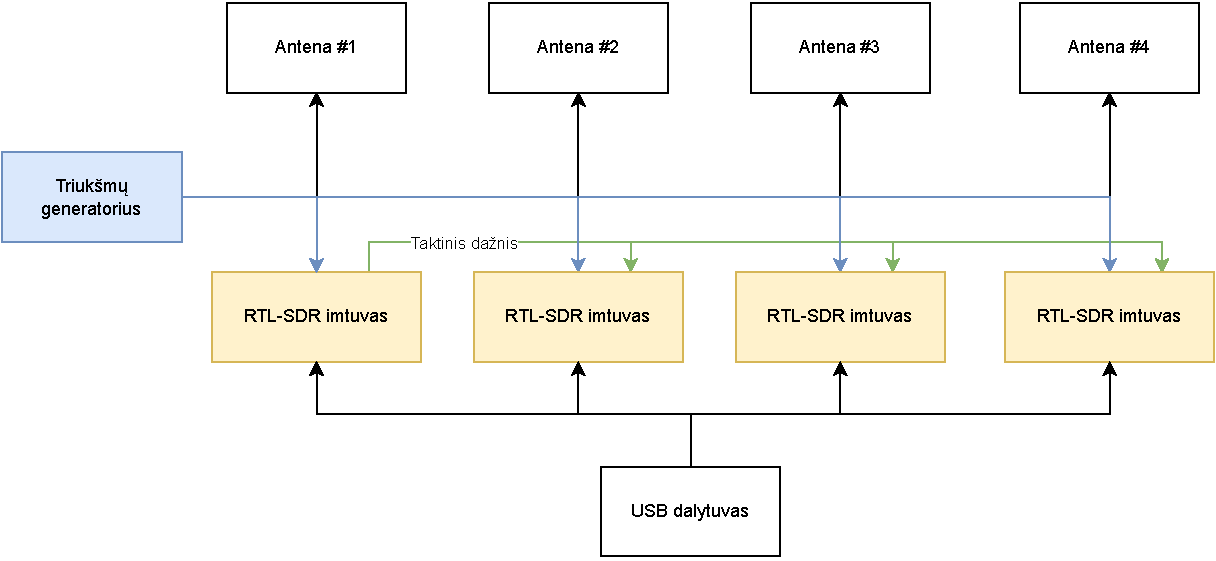
\includegraphics[scale=0.8]{drawings/kerberos_sdr_blockdiagram}
    \par\end{centering}
    \protect\caption{\label{fig:kerberos_block}KerberosSDR imtuvo blokinė diagrama.}
\end{figure}

\end{document}
